% Oficina de LaTeX (19.05.2008)
% Autor: Leandro Gutierrez Rizzi
% Exemplo 07

\documentclass[10pt]{article}
\usepackage{graphicx}
\usepackage{a4wide}

\pagestyle{empty}

\begin{document}

\renewcommand{\figurename}{Figura}

\begin{figure}[!t]
\centering
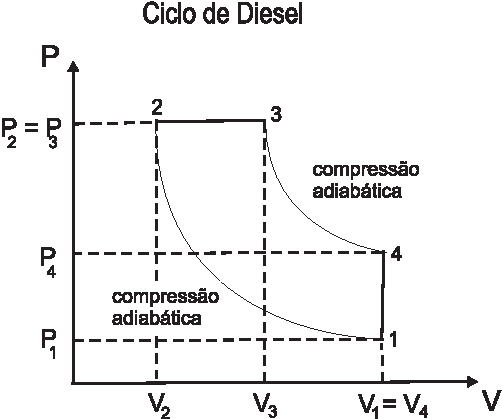
\includegraphics{diesel.eps}
\caption{Ciclo de diesel.}
\label{ciclodediesel}
\end{figure}

\begin{figure}[!b]
\centering
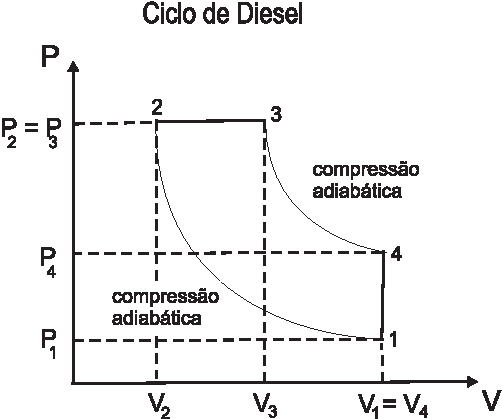
\includegraphics[width=0.50\textwidth]{diesel.eps}%
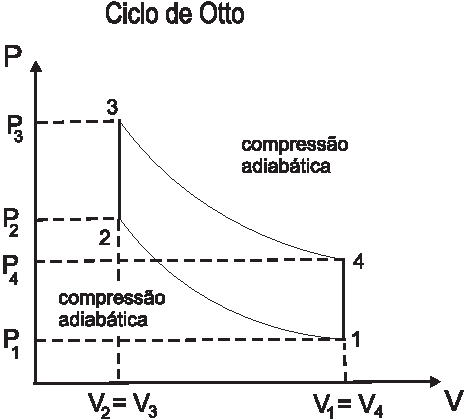
\includegraphics[width=0.462\textwidth]{otto.eps}
\caption{Ciclo de Diesel e Ciclo de Otto.}
\label{ciclodedieseleotto}
\end{figure}

\begin{figure}[h]
\flushleft
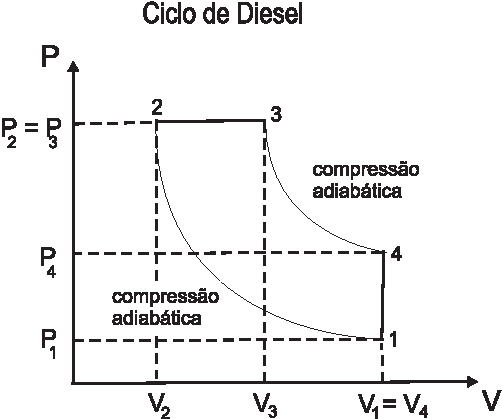
\includegraphics[width=0.70\textwidth]{diesel.eps}
\caption{Ciclo de Diesel.}
\label{ciclodedieseleotto1}

\vspace{1.0cm}

\hspace{0.6cm}
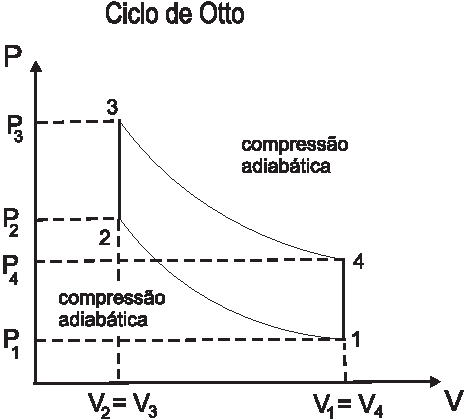
\includegraphics[width=0.70\textwidth]{otto.eps}
\caption{Ciclo de Otto.}
\label{ciclodedieseleotto2}
\end{figure}

\end{document}